\documentclass[a4paper,twoside]{article}
\usepackage[T1]{fontenc}
\usepackage[bahasa]{babel}
\usepackage{graphicx}
\usepackage{graphics}
\usepackage{float}
\usepackage[cm]{fullpage}
\pagestyle{myheadings}
\usepackage{etoolbox}
\usepackage{setspace} 
\usepackage{lipsum} 
\usepackage{caption}
\setlength{\headsep}{30pt}
\usepackage[inner=2cm,outer=2.5cm,top=2.5cm,bottom=2cm]{geometry} %margin
% \pagestyle{empty}
\usepackage[useregional=false]{datetime2}
\DTMsetdatestyle{ddmmyyyy}
\DTMsetup{datesep=/}
\usepackage{subcaption}
\renewcommand{\figurename}{Gambar} % change "Figure" to "Gambar"



\makeatletter
\renewcommand{\@maketitle} {\begin{center} {\LARGE \textbf{ \textsc{\@title}} \par} \bigskip {\large \textbf{\textsc{\@author}} }\end{center} }
\renewcommand{\thispagestyle}[1]{}
\markright{\textbf{\textsc{AIF234001/AIF234002 \textemdash Rencana Kerja Tugas Akhir \textemdash Sem. Ganjil 2023/2024}}}

\newcommand{\HRule}{\rule{\linewidth}{0.4mm}}
\renewcommand{\baselinestretch}{1}
\setlength{\parindent}{0 pt}
\setlength{\parskip}{6 pt}

\onehalfspacing

\begin{document}
	
	\title{\@judultopik}
	\author{\nama \textendash \@npm} 
	
	%tulis nama dan NPM anda di sini:
	\newcommand{\nama}{Arlo Dante Hananvyasa}
	\newcommand{\@npm}{6182201010}
	\newcommand{\@judultopik}{Pembangunan Perangkat Lunak dan Penyelesaian Permainan Colored Queens} % Judul/topik anda
	\newcommand{\jumpemb}{1} % Jumlah pembimbing, 1 atau 2
	\newcommand{\tanggal}{\DTMtoday}
	
	% Dokumen hasil template ini harus dicetak bolak-balik !!!!
	
	\maketitle
	
	\pagenumbering{arabic}
	
	\section{Deskripsi}
	Masalah \textit{n-queens} merupakan salah satu permasalahan klasik dalam ilmu komputer yang telah dipelajari secara ekstensif sejak abad ke-19. Permasalahan ini tergolong ke dalam kategori \textit{constraint satisfaction problem} (CSP), yaitu masalah yang melibatkan pencarian solusi dengan memberikan nilai pada elemen-elemen sedemikian rupa sehingga memenuhi sejumlah batasan atau kendala yang telah ditentukan, dan memiliki aplikasi luas dalam berbagai ruang lingkup seperti kecerdasan buatan dan teknik optimasi. Dalam bentuk standarnya, masalah \textit{n-queens} memerlukan penempatan $n$ buah bidak menteri pada papan catur berukuran $n \times n$ sedemikian rupa sehingga tidak ada menteri yang dapat menyerang satu sama lain secara horizontal, vertikal, dan diagonal tanpa batas jarak. Struktur permasalahan ini memenuhi definisi CSP yang mencakup: variabel berupa posisi setiap menteri, ruang solusi berupa kemungkinan kolom untuk setiap menteri, dan kendala berupa aturan tidak saling menyerang berdasarkan peraturan catur.
	
	\begin{figure}[H]
		\centering
		% increment the figure counter once for the whole group
		
		\begin{subfigure}{0.35\textwidth}
			\centering
			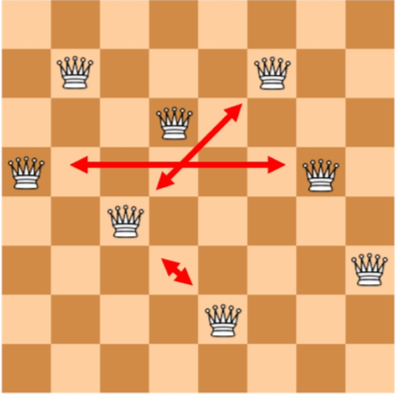
\includegraphics[width=\linewidth]{images/N_queens_wrong.png}
			\caption*{Gambar \thefigure(a) Contoh solusi salah masalah N-Queens}
			\label{fig:NQ_wrong}
		\end{subfigure}
		\hspace{2cm}
		\begin{subfigure}{0.35\textwidth}
			\centering
			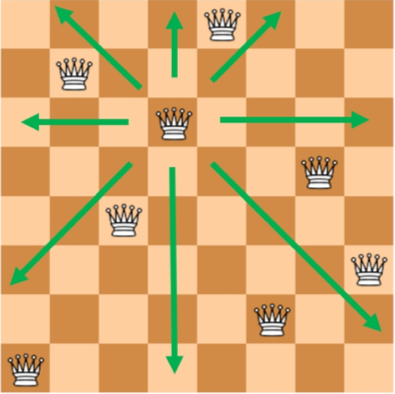
\includegraphics[width=\linewidth]{images/N_queens_correct.png}
			\caption*{Gambar \thefigure(b) Contoh valid permasalahan N-Queens}
			\label{fig:NQ_correct}
		\end{subfigure}
	\end{figure}
	
	
	Saat ini muncul berbagai variasi dari masalah n-queens tradisional. Salah satu varian yang menarik perhatian adalah Colored Queens, di mana papan permainan dibagi menjadi sektor-sektor berwarna dengan aturan tambahan bahwa setiap sektor harus berisi tepat satu menteri, dan tidak ada menteri yang boleh bersebelahan secara langsung baik horizontal, vertikal, maupun diagonal. Tidak seperti masalah n-queens tradisional, bidak menteri pada permainan Colored Queens hanya dapat menyerang secara horizontal dan vertikal, sehingga lebih dari satu bidak menteri dapat ditempatkan pada satu garis diagonal.

	\begin{figure}[H]
		\centering
 
		
		\begin{subfigure}{0.35\textwidth}
			\centering
			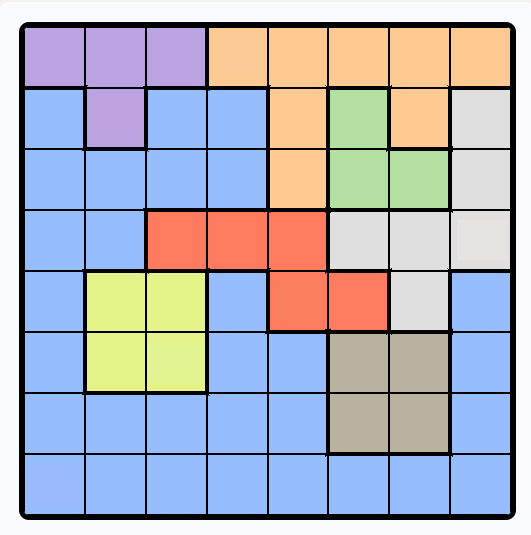
\includegraphics[width=\linewidth]{images/Queens_unsolved.png}
			\caption*{Gambar \thefigure(a) Contoh kondisi awal permainan Colored Queens}
			\label{fig:Queens_unsolved}
		\end{subfigure}
		\hspace{2cm}
		\begin{subfigure}{0.35\textwidth}
			\centering
			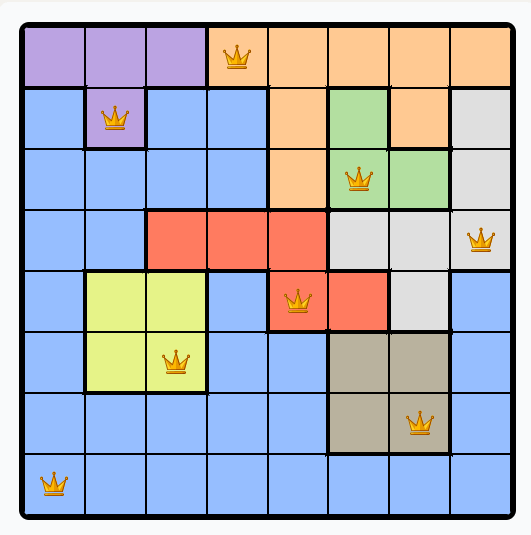
\includegraphics[width=\linewidth]{images/Queens_solved.png}
			\caption*{Gambar \thefigure(b) Solusi valid permainan Colored Queens}
			\label{fig:Queens_solved}
		\end{subfigure}
	\end{figure}
	
	Untuk menyelesaikan varian Colored Queens, penelitian ini akan menggunakan dua pendekatan algoritma yang berbeda, yaitu \textit{Backtracking} dan \textit{Particle Swarm Optimization} (PSO). Algoritma \textit{backtracking} merupakan pendekatan yang menggunakan pencarian mendalam dengan \textit{trial-and-error}, di mana solusi dibangun secara bertahap dan mundur ke keputusan sebelumnya ketika menemukan jalan buntu. Sementara itu, PSO adalah algoritma metaheuristik yang terinspirasi dari perilaku kawanan burung atau ikan dalam mencari makanan, menggunakan mekanisme kolaborasi antar partikel untuk mengeksplorasi ruang solusi. Karena permasalahan Colored Queens bersifat diskret sedangkan PSO dirancang untuk optimasi kontinu, diperlukan adaptasi khusus berupa diskretisasi posisi partikel dan mekanisme perbaikan untuk menangani solusi yang tidak valid. Kedua algoritma ini akan dibandingkan performanya untuk menentukan pendekatan mana yang lebih efektif dalam menyelesaikan permasalahan Colored Queens.
	
	Kompleksitas komputasional varian Colored Queens lebih tinggi dibanding permasalahan \textit{n-queens} tradisional karena terdapat kendala tambahan berupa aturan yang membatasi hanya satu bidak menteri pada setiap warna. Oleh karena itu, pendekatan \textit{Maintaining Arc Consistency} (MAC) yang mengimplementasikan algoritma \textit{Arc Consistency Algorithm 3} (AC-3) akan digunakan secara komplementer pada kedua algoritma tersebut. Peran AC-3 adalah untuk melakukan penyempitan ruang solusi berdasarkan batasan yang berlaku dengan mengeliminasi nilai-nilai yang tidak mungkin menghasilkan solusi valid. Algoritma AC-3 akan dijalankan pada tahap preprocessing dan selama proses pencarian berlangsung, sehingga ruang pencarian dapat dipersempit secara berkala dan efisiensi pencarian solusi meningkat secara signifikan.
	
	\begin{figure}[H]
		\centering
		
		\begin{subfigure}{0.35\textwidth}
			\centering
			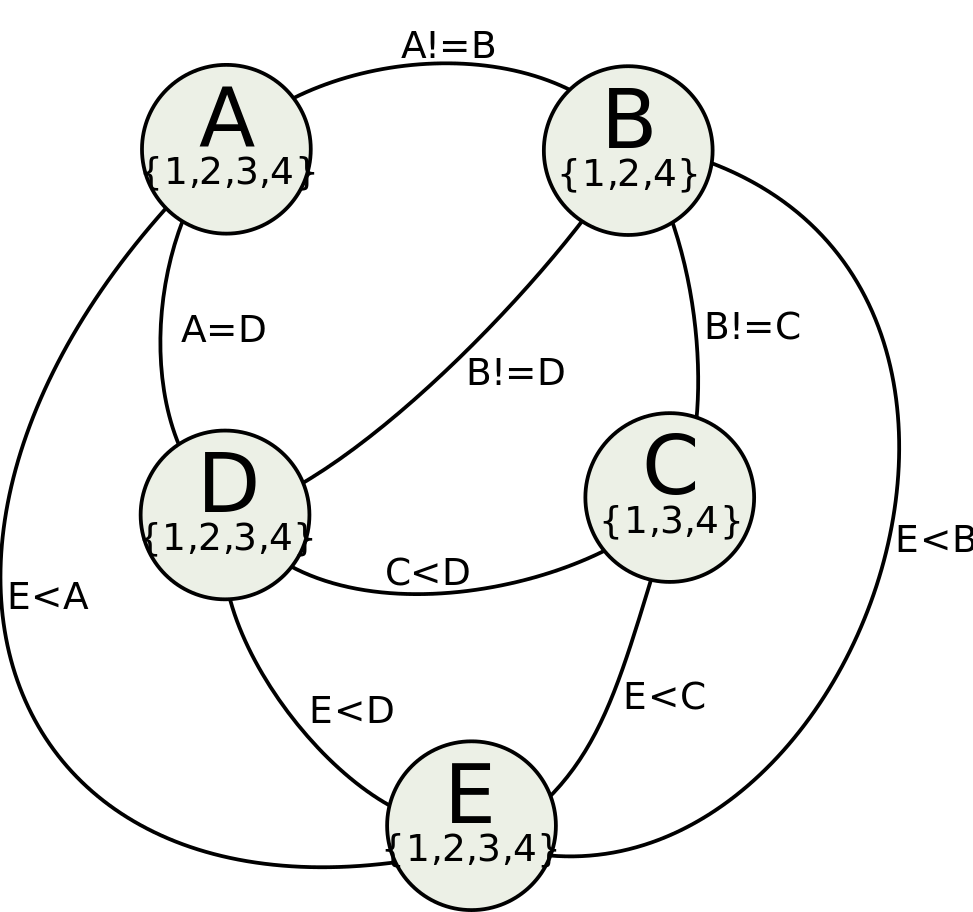
\includegraphics[width=\linewidth]{images/AC3_start.png}
			\caption*{Gambar \thefigure(a) Contoh ruang solusi variabel ABCDE sebelum algoritma AC-3}
			\label{fig:AC3_start}
		\end{subfigure}
		\hspace{2cm}
		\begin{subfigure}{0.35\textwidth}
			\centering
			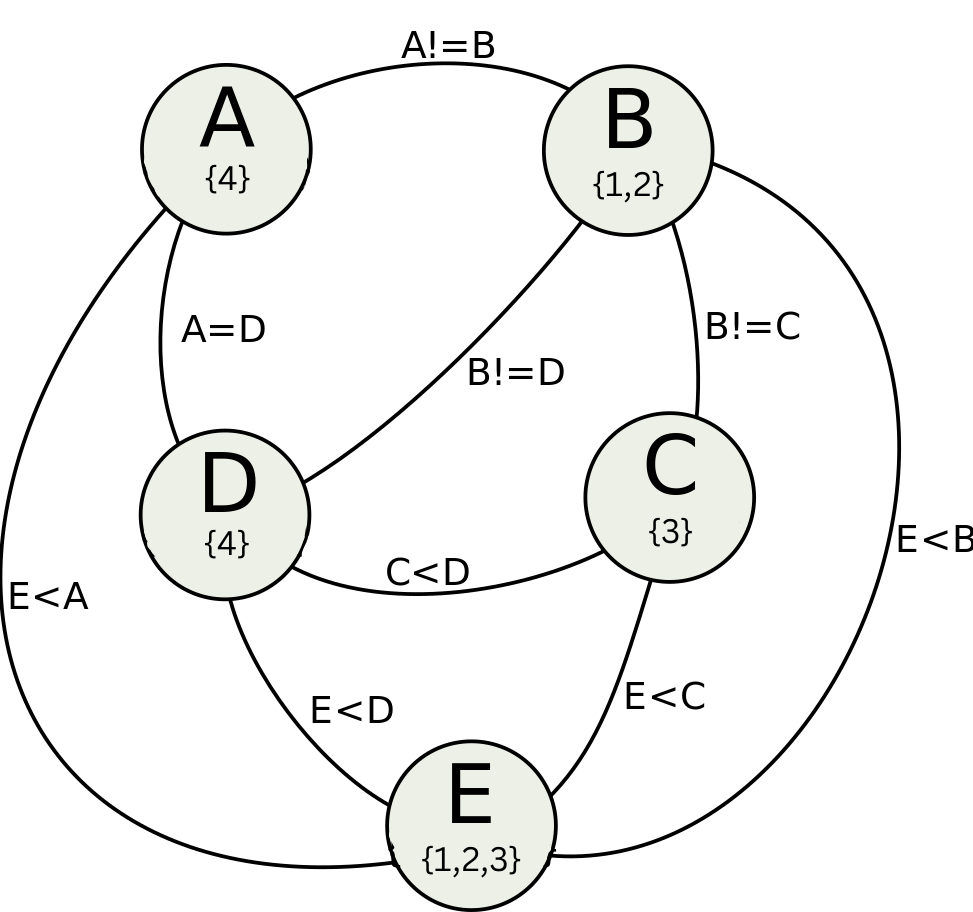
\includegraphics[width=\linewidth]{images/AC3_end.png}
			\caption*{Gambar \thefigure(b) Contoh ruang solusi variabel ABCDE setelah algoritma AC-3}
			\label{fig:AC3_end}
		\end{subfigure}
	\end{figure}
	
	
	Dari sisi pengembangan perangkat lunak, perancangan \textit{solver} untuk Colored Queens tidak hanya berfokus pada optimasi algoritma, tetapi juga pada penyediaan antarmuka pengguna yang intuitif dan mudah digunakan. Hal ini penting agar hasil solusi tidak hanya benar secara komputasional, tetapi juga dapat dipahami dan dimanfaatkan oleh pengguna tanpa beban kognitif yang berlebihan. Sebagai bagian dari tugas akhir ini, akan dirancang aplikasi berbasis web yang memungkinkan pengguna berinteraksi langsung dengan permainan Colored Queens, dilengkapi peringatan visual ketika terjadi pelanggaran kendala, serta fitur yang membantu memahami proses pencarian solusi yang dilakukan oleh sistem.
	
	\section{Rumusan Masalah}
	\begin{itemize}	
		\item Bagaimana cara membangun perangkat lunak permainan colored queens?
		
		\item Bagaimana membangun solusi permainan colored Queens menggunakan teknik \textit{Backtracking} dan \textit{Particle Swarm Optimization} (PSO)?
		
		\item Bagaimana membangun solver untuk permainan colored queen yang mengimplementasikan \textit{Backtracking} dan PSO yang dapat diintegrasikan dengan perangkat lunak yang dibangun?
		
		\item Bagiamana kinerja dari solver yang dibangun dalam mencari solusi permainan Colored Queens?
	\end{itemize}
	
	\section{Tujuan}
	\begin{itemize}	
		\item Membangun perangkat lunak permainan Colored Queens.
		
		\item Mempelajari cara membangun solusi permainan Colored Queen menggunakan teknik \textit{Backtracking} dan \textit{Particle Swarm Optimization}.
		
		\item Membangun solver untuk permainan colored queen yang mengimplementasikan \textit{Backtracking} dan PSO yang dapat diintegrasikan dengan perangkat lunak yang dibangun.
		
		\item Melakukan pegujian untuk mengukur kinerja dari solver yang dibangun dalam mencari solusi permainan Colored Queens
	\end{itemize}
	
	\section{Deskripsi Perangkat Lunak}
		\begin{itemize}
		\item Pengguna dapat memilih masalah Colored Queens yang ingin diselesaikannya yang sudah dikelompokan berdasarkan ukuran papan dan tingkat kesulitan.
		
		\item Pengguna dapat memainkan permainan Colored Queens untuk mencari solusi.
		
		\item Perangkat lunak akan memberikan peringatan pada pemain apabila menempatkan bidak menteri pada posisi yang invalid.
		
		\item Perangakat lunak dapat memberikan hint kepada pengguna apabila kesusahan dalam mencari solusi.
		
		\item Perangkat lunak dilengkapi oleh dua mode, yakni untuk permainan biasa dan untuk melakukan testing pencarian solusi menggunakan algoritma. Mode ini juga dilengkapi tampilan-tampilan penting seperti iterasi, waktu, dan perbandingan solusi yang ditemukan dan solusi-solusi yang diketahui
	\end{itemize}
	
	\section{Detail Pengerjaan Tugas Akhir}

	Bagian-bagian pekerjaan skripsi ini adalah sebagai berikut :
	\begin{enumerate}
		\item Melakukan studi literatur terkait permasalahan n-queens dan variannya, \textit{Constraint Satisfaction Problem} (CSP), algoritma pencarian Backtracking, teknik metaheuristik Particle Swarm Optimization, serta metode propagasi kendala AC-3.
		
		\item Mengumpulkan dan menyusun berbagai skenario permasalahan Colored Queens yang akan digunakan sebagai basis pengujian algoritma serta sebagai pilihan tingkat kesulitan bagi pengguna.
		
		\item Melakukan pemodelan masalah Colored Queens ke dalam bentuk CSP agar dapat diproses oleh algoritma pencarian.
		
		\item Melakukan analisis kebutuhan perangkat lunak, baik fungsional maupun non-fungsional, termasuk kebutuhan solver dan antarmuka pengguna.
		
		\item Merancang arsitektur sistem serta antarmuka pengguna untuk aplikasi \textit{Colored Queens Solver}.
		
		\item Mengimplementasikan algoritma Backtracking dan Particle Swarm Optimization dengan integrasi AC-3 sebagai mekanisme penyempitan ruang solusi.
		
		\item Melakukan pengujian efisiensi dan efektivitas algoritma (dengan dan tanpa AC-3) serta membandingkan kinerja metode Backtracking dan Particle Swarm Optimization.
		
		\item Mengembangkan antarmuka pengguna yang terhubung dengan solver untuk menampilkan visualisasi proses dan hasil pencarian solusi.
		
		\item Menyusun dokumentasi penelitian dan panduan penggunaan aplikasi.
	\end{enumerate}
	
	\section{Rencana Kerja}
	Rincian capaian yang direncanakan di Tugas Akhir 1 adalah sebagai berikut:
	\begin{enumerate}
		\item Melakukan studi literatur terkait permasalahan n-queens dan variannya, \textit{Constraint Satisfaction Problem} (CSP), algoritma pencarian Backtracking, teknik metaheuristik Particle Swarm Optimization, serta metode propagasi kendala AC-3.
		
		\item Mengumpulkan dan menyusun berbagai skenario permasalahan Colored Queens yang akan digunakan sebagai basis pengujian algoritma serta sebagai pilihan tingkat kesulitan bagi pengguna.
		
		\item Melakukan pemodelan masalah Colored Queens ke dalam bentuk CSP agar dapat diproses oleh algoritma pencarian.
		
		\item Melakukan analisis kebutuhan perangkat lunak, baik fungsional maupun non-fungsional, termasuk kebutuhan solver dan antarmuka pengguna.
		
		\item Merancang arsitektur sistem serta antarmuka pengguna untuk aplikasi \textit{Colored Queens Solver}.
		
		\item Menyusun dokumentasi tugas akhir untuk tahap TA 1.
	\end{enumerate}
	
	Sedangkan yang akan diselesaikan di Tugas Akhir 2 adalah sebagai berikut:
	\begin{enumerate}
		\item Mengimplementasikan algoritma Backtracking dan Particle Swarm Optimization dengan integrasi AC-3 sebagai mekanisme penyempitan ruang solusi.
		
		\item Melakukan pengujian efisiensi dan efektivitas algoritma (dengan dan tanpa AC-3) serta membandingkan kinerja metode Backtracking dan Particle Swarm Optimization.
		
		\item Mengembangkan antarmuka pengguna yang terhubung dengan solver untuk menampilkan visualisasi proses dan hasil pencarian solusi.
		
		\item Menyusun dokumentasi akhir, termasuk laporan penelitian dan panduan penggunaan aplikasi.
	\end{enumerate}
	
	\vspace{1cm}
	\centering Bandung, \tanggal\\
	\vspace{2cm} \nama \\ 
	\vspace{1cm}
	
	Menyetujui, \\
	\ifdefstring{\jumpemb}{2}{
		\vspace{1.5cm}
		\begin{centering} Menyetujui,\\ \end{centering} \vspace{0.75cm}
		\begin{minipage}[b]{0.35\linewidth}
			% \centering Bandung, \makebox[0.5cm]{\hrulefill}/\makebox[0.5cm]{\hrulefill}/2013 \\
			\vspace{2cm} Nama: \makebox[3cm]{\hrulefill}\\ Pembimbing Utama
		\end{minipage} \hspace{0.5cm}
		\begin{minipage}[b]{0.35\linewidth}
			% \centering Bandung, \makebox[0.5cm]{\hrulefill}/\makebox[0.5cm]{\hrulefill}/2013\\
			\vspace{2cm} Nama: \makebox[3cm]{\hrulefill}\\ Pembimbing Pendamping
		\end{minipage}
		\vspace{0.5cm}
	}{
		% \centering Bandung, \makebox[0.5cm]{\hrulefill}/\makebox[0.5cm]{\hrulefill}/2013\\
		\vspace{2cm} Nama: Husnul Hakim	\\ Pembimbing Tunggal
	}
\end{document}
